\label{ch:results}

\section{How the Depth Numbers Should Be Read}
Every depth label is the output of the rule engine, plus a little noise. A low error means the model has learned those rules. It does not mean a field trial measured emergence. The test set is a held-out portion of the same synthetic table. Random Forest importance puts crop identity at about 87\% of the split, which is expected: chickpea sits near 11\,cm and mustard near 4.5\,cm, so knowing the crop already explains most of the variance. Within a crop, Random Forest $R^{2}$ still runs from 0.72 for mustard to 0.95 for maize, so the remaining features are not empty. They are smaller than the crop effect.

\section{Single Split Served by the Application}
Table~\ref{tab:depth-one} is the run whose neural-network weights the website loads. The tree models were fit on the same split and are not served.

\begin{table}[H]
\centering
\caption{Test error on the single split used for the deployed depth network. Lower MAE is closer agreement with the rule labels.}
\label{tab:depth-one}
\begin{tabular}{lrr}
\toprule
\textbf{Model} & \textbf{Test MAE (cm)} & \textbf{Test $R^{2}$} \\
\midrule
Random Forest & 0.131 & 0.996 \\
XGBoost & 0.133 & 0.996 \\
AgroDynamicNet, all branches & 0.151 & 0.994 \\
AgroDynamicNet, crop only & 0.261 & 0.985 \\
AgroDynamicNet, soil only & 1.500 & 0.194 \\
AgroDynamicNet, weather only & 1.416 & 0.376 \\
\bottomrule
\end{tabular}
\end{table}

The trees are ahead of the network by about two tenths of a millimetre on this split. That gap is smaller than the 0.15\,cm noise added when the labels were built, so it is not a reason to prefer a tree in the product. The network is the model that can zero out a branch, which is why it is the one discussed in the ablation and the one loaded by the API. Soil alone and weather alone do not predict depth. Crop identity does. The useful question is the gap between crop-only and the full network.

Two further checks keep the single-split table from being read as a lucky test. On the training rows, five-fold cross-validation MAE is 0.141\,cm for the forest and 0.142\,cm for the boosted trees, each with a fold-to-fold standard deviation below 0.01\,cm. Those training figures sit close to the test figures in Table~\ref{tab:depth-one}. Inside the forest, the encoded crop name accounts for 0.874 of the impurity reduction. The next features are the seven-day rainfall, seed size and thousand-seed weight, each below 0.04. The boosted model also puts the crop first, and then the sowing month, which is tied to season. Within one crop the forest still has something to fit: $R^{2}$ runs from 0.72 on mustard to 0.95 on maize, with wheat at 0.80. The remaining features are real. They are much smaller than the jump from mustard at 4.5\,cm to chickpea at 11.25\,cm.

\section{Five Seeds and the Branch Ablation}
Five additional seeds were trained without replacing the deployed weights. Table~\ref{tab:depth-seeds} summarises them.

\begin{table}[H]
\centering
\caption{Five-seed depth results. The deployed weights are the earlier single run in Table~\ref{tab:depth-one}, whose MAE of 0.151\,cm sits inside the combined-network range below.}
\label{tab:depth-seeds}
\begin{tabular}{lrr}
\toprule
\textbf{Variant} & \textbf{Test MAE (cm)} & \textbf{Test $R^{2}$} \\
\midrule
Combined & $0.166 \pm 0.018$ & $0.994 \pm 0.001$ \\
Crop only & $0.256 \pm 0.009$ & $0.986 \pm 0.001$ \\
Soil only & $1.531 \pm 0.026$ & $0.171 \pm 0.028$ \\
Weather only & $1.418 \pm 0.025$ & $0.397 \pm 0.023$ \\
\bottomrule
\end{tabular}
\end{table}

Relative to the crop-only network, the combined network reduces MAE by 35.2\% on average. The arithmetic of that sentence is $(0.256 - 0.166) / 0.256$. The five seeds do not share the reduction equally. Table~\ref{tab:depth-by-seed} gives the test MAE of the combined network and of the crop-only network on each seed. The reduction is $(m_{\mathrm{crop}} - m_{\mathrm{full}}) / m_{\mathrm{crop}}$.

\begin{table}[H]
\centering
\caption{Test MAE in centimetres on each depth seed, to four decimal places. The reduction is computed from the unrounded errors and can differ in the second decimal from a ratio of the printed values. These runs did not replace the weights loaded by the API.}
\label{tab:depth-by-seed}
\begin{tabular}{rrrr}
\toprule
\textbf{Seed} & \textbf{Combined} & \textbf{Crop only} & \textbf{Reduction} \\
\midrule
0 & 0.1618 & 0.2477 & 34.7\% \\
1 & 0.1579 & 0.2549 & 38.0\% \\
2 & 0.1503 & 0.2673 & 43.8\% \\
3 & 0.1631 & 0.2469 & 33.9\% \\
4 & 0.1965 & 0.2632 & 25.3\% \\
\bottomrule
\end{tabular}
\end{table}

\begin{figure}[H]
\centering
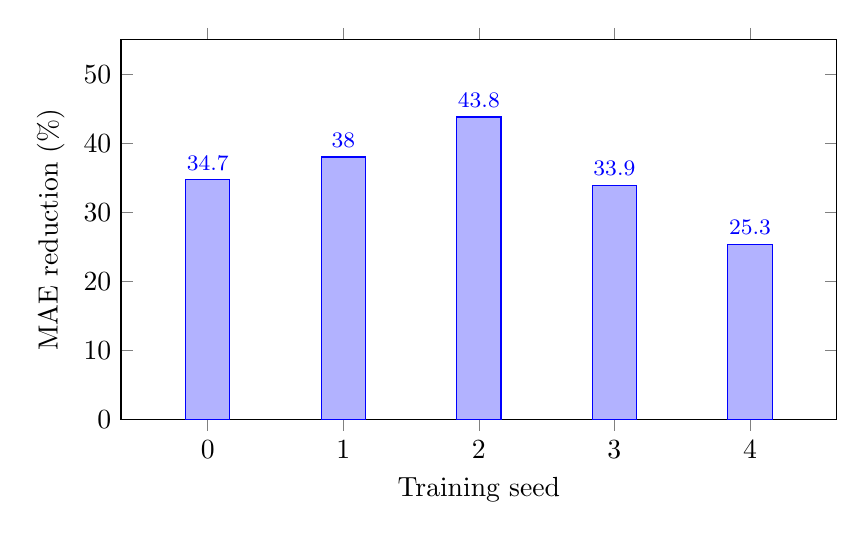
\begin{tikzpicture}
\begin{axis}[
    ybar,
    bar width=16pt,
    width=0.88\textwidth,
    height=6.4cm,
    ylabel={MAE reduction (\%)},
    xlabel={Training seed},
    symbolic x coords={0,1,2,3,4},
    xtick=data,
    ymin=0,
    ymax=55,
    nodes near coords,
    every node near coord/.append style={font=\footnotesize, /pgf/number format/fixed, /pgf/number format/precision=1},
    enlarge x limits=0.16,
    ytick={0,10,20,30,40,50},
]
\addplot coordinates {(0,34.7) (1,38.0) (2,43.8) (3,33.9) (4,25.3)};
\end{axis}
\end{tikzpicture}
\caption{Seed-wise reduction in test MAE when soil and weather are added to the crop-only network. The mean is 35.2\% and the sample standard deviation is 6.7 percentage points. Seed 4 is the low value.}
\label{fig:reduction}
\end{figure}

Four of the five seeds land between 0.1503 and 0.1631\,cm. Seed 4 lands at 0.1965\,cm, which is why the combined standard deviation is 0.018\,cm rather than a much smaller number. That seed is still 0.067\,cm closer to the labels than its own crop-only run, and it remains far below the soil-only and weather-only errors near 1.5\,cm. The study does not contain a seed in which adding soil and weather made the error worse. It does contain a seed whose gain is about 25\% rather than about 40\%, so the mean of 35.2\% should be quoted with the 6.7 point spread beside it. Soil alone ($R^{2}$ about 0.17) and weather alone ($R^{2}$ about 0.40) confirm that the gain is a joint effect. Neither branch is a hidden copy of the crop name.

Before the PAU range audit, on the same split, Random Forest was at 0.127\,cm / 0.989, XGBoost at 0.121\,cm / 0.990, the combined network at 0.153\,cm / 0.985 and the crop-only network at 0.208\,cm / 0.972. $R^{2}$ rose after the audit mostly because the crops moved further apart in depth. Those earlier reports are kept in the repository and are not the numbers the app should be quoted on.

\section{Vision-Model Pilot}
Forty photographs were drawn at random with a fixed seed: ten yellow rust, ten brown rust, ten powdery mildew and ten healthy. They were sent through the photo-check endpoint once. Nothing in the prompt was edited afterwards. Table~\ref{tab:pilot} records that pass. The interval is a 95\% interval on a sample of 30 diseased images, and it is wide.

\begin{table}[H]
\centering
\caption{Pilot of the PAU-list photo check on 40 John Innes Centre images. This pass does not use the ResNet18 score.}
\label{tab:pilot}
\begin{tabular}{lr}
\toprule
\textbf{Outcome} & \textbf{Count} \\
\midrule
Diseased images, correct first answer & 20 of 30 (67\%, interval 49--81\%) \\
Diseased images, correct disease in the top three & 21 of 30 (70\%, interval 52--83\%) \\
Diseased images with no match returned & 5 of 30 \\
Healthy images with no false alarm & 9 of 10 \\
\bottomrule
\end{tabular}
\end{table}

By class, the first answer was right for brown rust on 7 of 10, powdery mildew on 6 of 10, and yellow rust on 7 of 10. With ten images per class the intervals overlap, so the pilot does not show that one disease is easier. Five diseased images produced an empty list, which is a failure to help and also a refusal to invent a match.

\section{Fine-Tuned Classifiers}
ResNet18 and MobileNetV3-Small were fine-tuned on the other 959 images. The pilot files were excluded by hash before the split, so they are not in the 671 / 144 / 144 counts. Every seed reused that split. Table~\ref{tab:clf} is the five-seed summary.

\begin{table}[H]
\centering
\caption{Five-seed classifier results. Pilot columns count the 30 diseased and 10 healthy held-out photographs. Macro-F1 is on the 144-image test split.}
\label{tab:clf}
\small
\begin{tabular}{lrrrr}
\toprule
\textbf{Model} & \textbf{Accuracy} & \textbf{Macro-F1} & \textbf{Pilot, first} & \textbf{Pilot, healthy} \\
\midrule
ResNet18 & $89.4\% \pm 2.2\%$ & $0.880 \pm 0.023$ & $25.2 \pm 1.3$ of 30 & 9 of 10 \\
MobileNetV3-Small & $75.3\% \pm 1.9\%$ & $0.735 \pm 0.015$ & $24.4 \pm 1.8$ of 30 & $8.8 \pm 0.4$ of 10 \\
\bottomrule
\end{tabular}
\end{table}

On this pilot the vision model's 20 of 30 sits below both means. The comparison favours the classifiers: they trained on the same dataset the pilot photographs come from, and the vision model did not. Thirty diseased photographs are enough to make the gap suggestive and not enough to make it precise. CerealConv's 97.05\% \cite{long2023wheat} is a result on a different protocol and a larger training set. It is not a number KrishiBee missed.

The five ResNet18 seeds are not interchangeable in detail, which is why the mean is reported with a standard deviation. Test accuracy runs from 0.875 on seeds 2 and 4 to 0.924 on seed 3. Macro-F1 runs from 0.857 to 0.915. On the 30 diseased pilot images the seeds score 27, 24, 24, 25 and 26, so the mean of 25.2 has a standard deviation of 1.3 images. Healthy images are 9 of 10 on every seed. MobileNetV3-Small stays near 75\% accuracy and near 0.735 macro-F1, and its healthy count is the only one that moves, at $8.8 \pm 0.4$ of 10. The smaller network is a useful baseline and a poor candidate for the page. The page loads seed 0 of ResNet18, whose accuracy of 0.8889 and macro-F1 of 0.8785 sit inside the five-seed band and slightly below the mean. Choosing the seed with the highest test accuracy after looking at the test split would have inflated the number the farmer sees. That was not done.

The validation temperature of that checkpoint is 0.8484. A temperature below 1 sharpens the distribution: probabilities move away from 0.5, so a class that was already ahead becomes more confident. Expected calibration error, computed in ten equal-width bins, moves from 0.0831 to 0.0712. The change is modest. The operating point does more work than the scaling. At a threshold of 0.5 the seed-0 test keeps 95.1\% of images and is right on 91.2\% of those it keeps. At 0.7 the coverage is 81.9\% and the accuracy is 94.9\%. At 0.8 the coverage is 68.1\% and the accuracy is 95.9\%. At 0.9 the coverage falls to 54.2\% and the accuracy is 94.9\%, a little below the accuracy at 0.8. On 144 images that reversal is a small-sample fact, recorded in Table~\ref{tab:coverage}, and it is not a claim that a stricter threshold is worse in general. The threshold shown to the farmer is 0.8. It names about two thirds of the test images, and the names it keeps are right about 96\% of the time on this split. The coarser summary ``about 70\% coverage and about 95\% accuracy'' is this table, read loosely.

\section{Four Photographs on the Deployed Classifier}
The 40-image pilot has no septoria folder. Septoria remains one of the five classes in the 144-image test split. As a separate check of the deployed card, one image from each pilot folder was sent through the running photo check. Table~\ref{tab:spot} is that check. It is an illustration of the threshold, not a second test set.

\begin{table}[H]
\centering
\caption{One photograph from each pilot class, scored by the deployed ResNet18. A probability below 0.8 is withheld even when the top class is the folder name.}
\label{tab:spot}
\begin{tabular}{llcc}
\toprule
\textbf{File} & \textbf{Top class} & \textbf{Probability} & \textbf{Shown} \\
\midrule
\texttt{brown-rust\_00} & Brown rust & 0.964 & Named \\
\texttt{yellow-rust\_00} & Yellow rust & 0.851 & Named \\
\texttt{healthy\_00} & Healthy & 0.996 & Named \\
\texttt{powdery-mildew\_00} & Powdery mildew & 0.606 & Withheld \\
\bottomrule
\end{tabular}
\end{table}

The powdery-mildew case is the important row. The top class matches the folder and the page still refuses to name it. On that same photograph the PAU-list path described white floury spots and matched powdery mildew. The two paths are allowed to disagree in confidence. The farmer sees both.

\screenshot{figures/photo-named.png}{Photo check on a brown-rust pilot image. The ResNet18 name is shown because the probability is above 0.8.}{fig:photo-named}

\screenshot{figures/photo-withheld.png}{Photo check on the powdery-mildew pilot image. The top class is correct and the probability is 0.606, so the name is withheld.}{fig:photo-withheld}

\section{One Session on the Deployed Site}
The tables above are the evaluation. This section is one pass through the public site, made so that those tables can be pointed at on a screen. The field was a point in Punjab, the crop was wheat, and the season was Rabi. SoilGrids did not answer. The card said that cached soil from 23.0\,km away had been used. The derived texture was loam and the estimated moisture was 24.43\%. The network depth was 4.95\,cm. The rule depth was 4.88\,cm. The safe range printed beside them was 4--6\,cm.

The rule figure is the arithmetic of Chapter~\ref{ch:design}. Wheat starts at an optimal depth of 5.0\,cm. Loam adds nothing. Moisture near 24\% adds about $-0.12$\,cm. The result rounds to 4.88\,cm when the rain and temperature terms are zero. The network is 0.07\,cm away. That is inside the 0.151\,cm test MAE of the deployed weights, and it is not a germination measurement. The cached soil is a real degradation: the texture and moisture are from a point 23\,km away, and the card says so.

The forecast on the same date, 28 October 2026, named rain as likely on 30 October and named the next open task as the weed-control window, then running from 20 October to 4 November. That task is not an irrigation, so the card did not add the ``check the field before you irrigate'' sentence. A later week, or a different sowing date, would. The forecast is not scored in Table~\ref{tab:depth-one} and is not an input to the network.

The chat was asked when to give the first irrigation. The reply placed a light first irrigation after the crop had started to grow, at about three weeks for an early-October sowing and about four weeks for a sowing from mid-October to early November, and it referred to the Punjab loam and the estimated moisture. That is the timetable the ungrounded bot had missed. The page still carries the standing warning that answers are drawn from a small set of notes and that quantities should be confirmed with the KVK. The prose can add a clause that is not in the note. The source line under the answer is what the farmer, and an examiner, should read.

\section{Screens of the Deployed Advisor}
The following figures record the requirements in Table~\ref{tab:fr} on the running site at \url{https://krishi-bee.vercel.app}.

\screenshot{figures/depth.png}{Depth advisor for wheat in Punjab. The card shows the network depth, the rule depth and the 4--6\,cm range together.}{fig:depth}

\screenshot{figures/forecast.png}{Seven-day forecast under the map, including the line that names the next open task.}{fig:forecast}

\screenshot{figures/chat.png}{A sourced answer on first irrigation, with the PAU note listed under the reply.}{fig:chat}

\screenshot{figures/tracker.png}{Wheat calendar after a sowing date, with task windows counted from that date.}{fig:tracker}

\section{Discussion}
The depth result that should be quoted is not the $R^{2}$ of 0.994. Crop identity makes a high $R^{2}$ easy once chickpea and mustard sit far apart. The result that should be quoted is the 0.09\,cm gap between the crop-only MAE and the combined MAE, repeated over five seeds, together with the statement that the labels are rules. The trees winning by a fraction of a millimetre does not change the product decision. The network is what makes the ablation the same model as the deployment.

The classifier result that should be quoted is the pair of coverage and accuracy at 0.8, plus the pilot comparison, plus the geography. A system that names every image at 89\% accuracy would be a worse fit for this interface than a system that names about two thirds of them and is right about 96\% of the time on the test split. The withheld powdery-mildew photograph is the demonstration of that choice.

The forecast has no accuracy table. It is a pass-through of a public forecast, joined to a task the calendar already knew. Its failure mode on the hosted API, and the move into the browser, belong in the report because they change which component the farmer is actually calling.

What the project does not show is a germination count, a Punjab leaf, or a second season of use. Those are the limits in the next chapter, and they are already the limits of the evidence above.
